\documentclass[tikz,border=6pt]{standalone}
\usepackage{tikz}
\begin{document}
\small
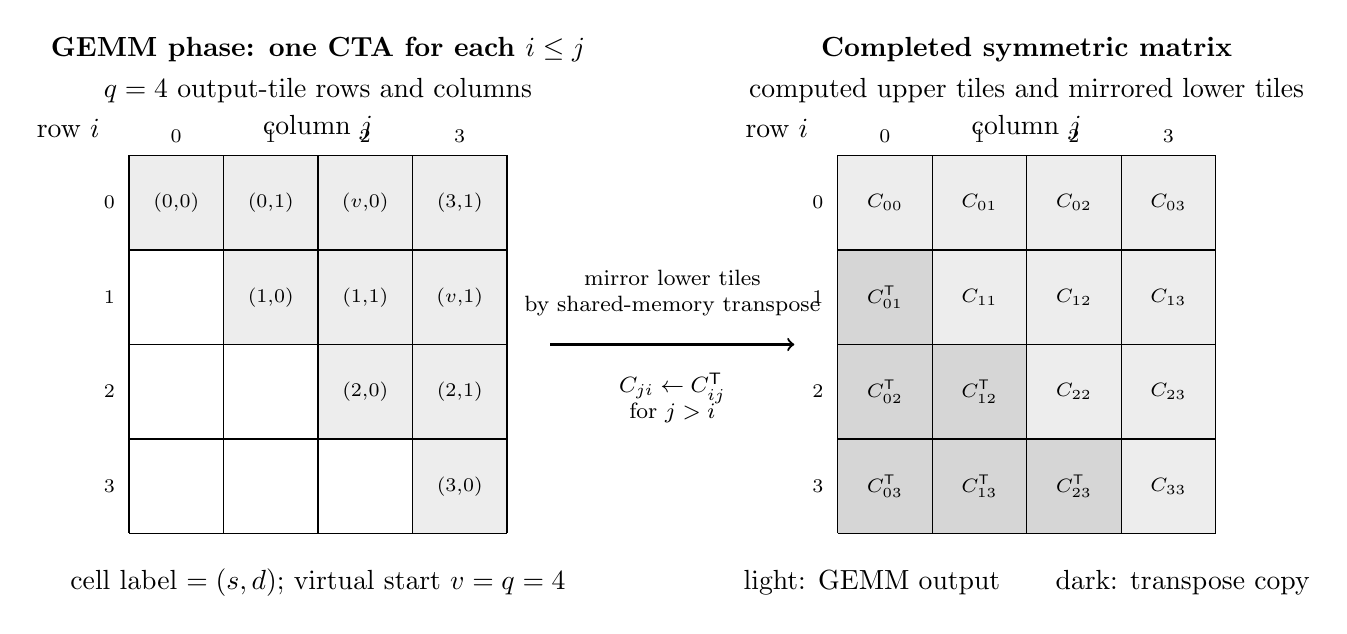
\begin{tikzpicture}
  \node[font=\bfseries] at (2.4,1.35) {GEMM phase: one CTA for each $i\le j$};
  \node at (2.4,0.82) {$q=4$ output-tile rows and columns};
  \node[anchor=east] at (-0.25,0.35) {row $i$};
  \node at (2.4,0.35) {column $j$};

  \fill[gray!14] (0,0) rectangle (4.8,-1.2);
  \fill[gray!14] (1.2,-1.2) rectangle (4.8,-2.4);
  \fill[gray!14] (2.4,-2.4) rectangle (4.8,-3.6);
  \fill[gray!14] (3.6,-3.6) rectangle (4.8,-4.8);

  \foreach \gridline in {0,...,4} {
    \draw ({1.2*\gridline},0) -- ({1.2*\gridline},-4.8);
    \draw (0,{-1.2*\gridline}) -- (4.8,{-1.2*\gridline});
  }
  \foreach \index in {0,...,3} {
    \node at ({1.2*\index+0.6},0.25) {$\scriptstyle \index$};
    \node at (-0.25,{-1.2*\index-0.6}) {$\scriptstyle \index$};
  }

  \node at (0.6,-0.6) {$\scriptstyle(0,0)$};
  \node at (1.8,-0.6) {$\scriptstyle(0,1)$};
  \node at (3.0,-0.6) {$\scriptstyle(v,0)$};
  \node at (4.2,-0.6) {$\scriptstyle(3,1)$};
  \node at (1.8,-1.8) {$\scriptstyle(1,0)$};
  \node at (3.0,-1.8) {$\scriptstyle(1,1)$};
  \node at (4.2,-1.8) {$\scriptstyle(v,1)$};
  \node at (3.0,-3.0) {$\scriptstyle(2,0)$};
  \node at (4.2,-3.0) {$\scriptstyle(2,1)$};
  \node at (4.2,-4.2) {$\scriptstyle(3,0)$};

  \node[align=center] at (2.4,-5.42)
    {cell label $=(s,d)$; virtual start $v=q=4$};

  \draw[->,line width=0.8pt] (5.35,-2.4) -- (8.45,-2.4);
  \node[align=center,font=\footnotesize] at (6.9,-1.75) {mirror lower tiles\\by shared-memory transpose};
  \node[align=center,font=\footnotesize] at (6.9,-3.08) {$C_{ji}\leftarrow C_{ij}^{\mathsf T}$\\for $j>i$};

  \node[font=\bfseries] at (11.4,1.35) {Completed symmetric matrix};
  \node at (11.4,0.82) {computed upper tiles and mirrored lower tiles};
  \node[anchor=east] at (8.75,0.35) {row $i$};
  \node at (11.4,0.35) {column $j$};

  \fill[gray!14] (9.0,0) rectangle (13.8,-1.2);
  \fill[gray!14] (10.2,-1.2) rectangle (13.8,-2.4);
  \fill[gray!14] (11.4,-2.4) rectangle (13.8,-3.6);
  \fill[gray!14] (12.6,-3.6) rectangle (13.8,-4.8);
  \fill[gray!32] (9.0,-1.2) rectangle (10.2,-2.4);
  \fill[gray!32] (9.0,-2.4) rectangle (11.4,-3.6);
  \fill[gray!32] (9.0,-3.6) rectangle (12.6,-4.8);

  \foreach \gridline in {0,...,4} {
    \draw ({9.0+1.2*\gridline},0) -- ({9.0+1.2*\gridline},-4.8);
    \draw (9.0,{-1.2*\gridline}) -- (13.8,{-1.2*\gridline});
  }
  \foreach \index in {0,...,3} {
    \node at ({9.0+1.2*\index+0.6},0.25) {$\scriptstyle \index$};
    \node at (8.75,{-1.2*\index-0.6}) {$\scriptstyle \index$};
  }

  \node at (9.6,-0.6) {$\scriptstyle C_{00}$};
  \node at (10.8,-0.6) {$\scriptstyle C_{01}$};
  \node at (12.0,-0.6) {$\scriptstyle C_{02}$};
  \node at (13.2,-0.6) {$\scriptstyle C_{03}$};
  \node at (9.6,-1.8) {$\scriptstyle C_{01}^{\mathsf T}$};
  \node at (10.8,-1.8) {$\scriptstyle C_{11}$};
  \node at (12.0,-1.8) {$\scriptstyle C_{12}$};
  \node at (13.2,-1.8) {$\scriptstyle C_{13}$};
  \node at (9.6,-3.0) {$\scriptstyle C_{02}^{\mathsf T}$};
  \node at (10.8,-3.0) {$\scriptstyle C_{12}^{\mathsf T}$};
  \node at (12.0,-3.0) {$\scriptstyle C_{22}$};
  \node at (13.2,-3.0) {$\scriptstyle C_{23}$};
  \node at (9.6,-4.2) {$\scriptstyle C_{03}^{\mathsf T}$};
  \node at (10.8,-4.2) {$\scriptstyle C_{13}^{\mathsf T}$};
  \node at (12.0,-4.2) {$\scriptstyle C_{23}^{\mathsf T}$};
  \node at (13.2,-4.2) {$\scriptstyle C_{33}$};

  \node[align=center] at (11.4,-5.42)
    {light: GEMM output\qquad dark: transpose copy};
\end{tikzpicture}
\end{document}
